\documentclass[10pt,letterpaper]{article}
\usepackage[top=0.85in,left=2.75in,footskip=0.75in]{geometry}

% amsmath and amssymb packages, useful for mathematical formulas and symbols
\usepackage{amsmath,amssymb}

% Use adjustwidth environment to exceed column width (see example table in text)
\usepackage{changepage}

% Use Unicode characters when possible
\usepackage[utf8x]{inputenc}

% textcomp package and marvosym package for additional characters
\usepackage{textcomp,marvosym}

% cite package, to clean up citations in the main text. Do not remove.
\usepackage{cite}

% Use nameref to cite supporting information files (see Supporting Information section for more info)
\usepackage{nameref,hyperref}

% line numbers
\usepackage[right]{lineno}

% ligatures disabled
\usepackage{microtype}
\DisableLigatures[f]{encoding = *, family = * }

% color can be used to apply background shading to table cells only
\usepackage[table]{xcolor}

% array package and thick rules for tables
\usepackage{array}

% enumerate package lets us use letters instead of numbers
\usepackage{enumerate}

% create "+" rule type for thick vertical lines
\newcolumntype{+}{!{\vrule width 2pt}}

% create \thickcline for thick horizontal lines of variable length
\newlength\savedwidth
\newcommand\thickcline[1]{%
  \noalign{\global\savedwidth\arrayrulewidth\global\arrayrulewidth 2pt}%
  \cline{#1}%
  \noalign{\vskip\arrayrulewidth}%
  \noalign{\global\arrayrulewidth\savedwidth}%
}

% \thickhline command for thick horizontal lines that span the table
\newcommand\thickhline{\noalign{\global\savedwidth\arrayrulewidth\global\arrayrulewidth 2pt}%
\hline
\noalign{\global\arrayrulewidth\savedwidth}}

\usepackage{color}

% Remove comment for double spacing
%\usepackage{setspace}
%\doublespacing

% Text layout
\raggedright
\setlength{\parindent}{0.5cm}
\textwidth 5.25in
\textheight 8.75in

% Bold the 'Figure #' in the caption and separate it from the title/caption with a period
% Captions will be left justified
\usepackage[aboveskip=1pt,labelfont=bf,labelsep=period,justification=raggedright,singlelinecheck=off]{caption}
\renewcommand{\figurename}{Fig}

% Use the PLoS provided BiBTeX style
\bibliographystyle{plos2015}

% Remove brackets from numbering in List of References
\makeatletter
\renewcommand{\@biblabel}[1]{\quad#1.}
\makeatother

% Leave date blank
\date{}

% Header and Footer with logo
\usepackage{lastpage,fancyhdr,graphicx}
\usepackage{epstopdf}
\pagestyle{myheadings}
\pagestyle{fancy}
\fancyhf{}
\setlength{\headheight}{27.023pt}
\lhead{
\includegraphics[width=2.0in]{PLOS-submission.eps}}
\rfoot{\thepage/\pageref{LastPage}}
\renewcommand{\footrule}{\hrule height 2pt \vspace{2mm}}
\fancyheadoffset[L]{2.25in}
\fancyfootoffset[L]{2.25in}
\lfoot{\sf PLOS}


\newcommand{\rulemajor}[1]{\section*{#1}}
\newcommand{\withurl}[2]{{#1}\footnote{{\texttt{#2}}}}

\begin{document}
\vspace*{0.2in}

\begin{flushleft}
{\Large
\textbf\newline{Ten Simple Rules for Helping Newcomers Become Contributors to Open Source Projects}
}
\newline
\\
{Mara Averick}\textsuperscript{1{\ddag}},
{Denae Ford}\textsuperscript{2{\ddag}},
{Mike Hoye}\textsuperscript{3{\ddag}},
{Dan Sholler}\textsuperscript{4{\ddag}},
{Igor Steinmacher}\textsuperscript{5{\ddag}},
{Greg Wilson}\textsuperscript{1{\ddag}*}
\\
\bigskip
\textbf{1} RStudio, Inc. / \{mara.averick, greg.wilson\}@rstudio.com \\
\textbf{2} North Carolina State University / dford3@ncsu.edu \\
\textbf{3} Mozilla Corporation / mhoye@mozilla.com \\
\textbf{4} Berkeley Institute for Data Science / sholler.daniel@gmail.com \\
\textbf{5} Northern Arizona University/ igor.steinmacher@nau.edu \\\bigskip
* Corresponding author. \\
\bigskip
{\ddag} These authors contributed equally to this work.
\end{flushleft}

\section*{Abstract}

In order to survive and thrive,
a community needs to attract and retain new members
and help them be productive.
The 10 simple rules outlined in this paper
summarize best practices for doing this
that are evidence-based and have demonstrated their effectiveness
in a wide variety of open source and open science projects.

\section*{Author Summary}

Research has always been a communal activity,
but researchers have only recently begun to pay attention to
what we know know about why some communities thrive and others fail.
Attracting contributors,
retaining them,
and helping them be more productive
have all been the subject of intensive study.
This paper presents 10 findings from those studies that community leaders can apply immediately
and explains why they work.

\section*{Introduction}

In order to survive and thrive,
a community needs to attract new members,
retain them,
and help them be productive contributors.
As openness becomes the norm in scientific research and software development,
knowing how to do this has become a necessary skill for principal investigators and other project leaders.
While every situation is unique,
A growing body of knowledge in sociology, anthropology, education, and software engineering
can guide decisions about what to do to facilitate this.

But what exactly do we mean by ``community''?
In the case of open source and open science,
the most usual meaning is a ``community of practice''.
As defined by Lave and Wenger~\cite{lave1991,wenger1999},
these have three key characteristics:

\begin{enumerate}

\item Participants have a common purpose or product that they work on or toward.

\item They are mutually engaged, i.e., they assist and mentor each another.

\item They develop shared resources and domain knowledge.

\end{enumerate}

By analogy,
Brown~\cite{brown2019} defines a ``community of effort'' as,
``{\ldots}a community formed in pursuit of a common goal.
The goal can be definite or indefinite in time,
and may not be clearly defined,
but it's something that (generally speaking) the community is aligned on.''
An open source software projects like Mozilla Firefox~\cite{mozilla} is one example:
a mix of paid professionals,
highly-involved volunteers,
and occasional passers by create software,
documentation,
and tutorials
while also organizing events,
answering questions in online forums,
mentoring newcomers,
and advocating for open standards.

People working to preserve coral reefs in the face of global climate change are an example of
a more loosely connected community of effort.
There is no single central organization coordinating their work,
but the scientists who study coral reefs,
the environmentalists who work to protect them,
and the citizens who support them financially and politically
are aware of each other's efforts,
coordinate with each other in various ad hoc ways,
and are conscious of contributing toward a shared purpose.

Every community of effort has its own unique features,
but they have enough in common to profit from one another's experience.
The 10 rules laid out below are based on studies of such communities
and on the authors' experience as members,
leaders,
and observers of them.

\rulemajor{Rule 1: have and enforce a code of conduct.}

The first and most important rule is
to explicitly codify guidelines for all members of the community to follow
to foster an environment that newcomers find healthy and welcoming.
An increasingly popular strategy for doing so is to adopt and publish a Code of Conduct.
Many projects such as rOpenSci~\cite{ropensci-coc},
NumPy~\cite{numpy-coc},
and Project Jupyter~\cite{jupyter-coc}
have adopted Codes of Conduct
based on the Contributor Covenant~\cite{covenant}
or other frameworks such as SciPy's Code of Conduct~\cite{scipy-coc}.

However, several questions around reporting violations and enforcing rules remain open.
What is the appropriate mechanism for reporting violations?
Who should receive reports?
What types of actions can projects take when a member of the community violates the code?
Projects may vary in how they address these questions based on characteristics of size, technology choices, or human resources
(such as the presence of a community manager).
However, some must-haves are clear based on our collective experience and code of conduct guides~\cite{aurora2019}.

For instance,
projects should designate at least one independent party
(i.e., an individual not employed by or otherwise deeply tied the project)
to receive and review reports.
An independent party offers a degree of objectivity
and can help to protect reporters from hesitating to report out of fear of retribution or damage to their reputation.
When possible,
the independent party should be part of a more extensive code of conduct committee made up of several people with varied characteristics
(e.g., gender identity, race, ethnicity, roles in the community).
Any member of the committee implicated in the incident should be recused from reviewing the violations.

Project leaders should also develop some enforcement mechanisms and,
when safe for the reporter,
publicize the enforcement decision.
Enforcing the code and announcing decisions are critical;
otherwise,
the community will quickly recognize the code as meaningless.
Committees can consider several courses of action once investigations are complete:
verbal or written warnings,
limits on access to project communication avenues (e.g., Slack channels or mailing lists),
or in severe cases,
suspension or expulsion from contributing to the project.

\rulemajor{Rule 2: Make governance explicit.}

Raymond's ``The Cathedral and the Bazaar''~\cite{raymond2001}
was one of the most influential documents in the history of open source.
It described an egalitarian world in which everyone could contribute equally to the greater good,
but as Bezroukov pointed out~\cite{bezroukov1999},
that description ignored the realities of how power arises,
becomes concentrated in a few hands,
and is then used to perpetuate itself.
Bezroukov's criticism drew on Freeman's influential essay ``The Tyranny of Structurelessness''~\cite{freeman1972},
which explained how an apparent lack of structure in organizations ``{\ldots}too often disguised an informal,
unacknowledged and unaccountable leadership that was all the more pernicious because its very existence was denied.''

Two decades later,
we can see how unequal and unwelcoming the supposedly egalitarian ``bazaar'' of open source can be
if authority lies with those willing to shout loudest and longest.
Making a project's governance explicit is therefore essential to making that project inviting and welcoming to newcomers with diverse backgrounds.
The most basic way to do this is to adopt something like the Contributor Covenant~\cite{covenant},
which lays out ground rules for interpersonal interaction within the project.
At the opposite end,
large, well-established projects that incorporate as non-profits are required to promulgate bylaws,
such as those for the Python Software Foundation~\cite{psf-bylaws}.

What lies between these two extremes is less well documented,
but the ``Social and Political Infrastructure'' chapter of~\cite{fogel2005} is a good place to start.
It describes two models:

\begin{itemize}
	
\item
  A \emph{benevolent dictator} (who might better be called a ``community-approved arbitrator'') has final say,
  but their principal responsibility is to manage conversation to achieve consensus.
	
\item
  When consensus cannot be achieved,
  organizations may hold a vote.
  Organizations should decide who is and isn't eligible to vote well in advance of the emergence of issues requiring votes,
  since tempers may already be running hot by the time this point is reached.
  In the Carpentries,
  for example,
  anyone who satisfies any of the conditions below is eligible to run for a seat on the Executive Council
  and to vote in those elections~\cite{carpentries-bylaws}:
  \begin{enumerate}
  \item
    everyone who has completed instructor certification in the preceding year;
  \item
    everyone who has completed certification in the last two years and taught at least one workshop;
  \item
    everyone who has been certified for more than two years and has taught at least twice in that time; and
  \item
    anyone who has made a significant contribution to lesson development, infrastructure, or other activities
    as determined by the Executive Council.
  \end{enumerate}

\end{itemize}

No organization wants to become mired in red tape of its own making,
but equally no one has ever said,
``I wish we had waited longer before making our rules explicit.''
Should any reader wish to make a significant non-coding contribution to open source,
a series of three or four successively more elaborate models for governance,
each annotated to explain when and why the extra complexity should be added, would be extremely valuable.

\rulemajor{Rule 3: Make it clear that newcomers are welcome.}

Perhaps the most obvious of the methods for making newcomers feel welcome is to greet them with kindness and politeness.
A newcomer's first impression of a project will influence their perceptions of the project's overall environment
and in turn their likelihood to sustain engagement with the project.
As Fogel said~\cite{fogel2005},
``If a project doesn't make a good first impression, newcomers may wait a long time before giving it a second chance.''
Other authors have empirically evaluated and confirmed the importance of kind and polite social environments
in open source projects \cite{singh2012,steinmacher2013,steinmacher2018}.
Therefore,
extra steps
(beyond following the basic guidelines set forth in the Code of Conduct)
should be taken to foster a positive feeling.
Several approaches can be taken, including:

\begin{itemize}

\item
  Posting a welcome message on the project's social media pages, Slack channels, forums, or email lists.
  Projects might consider maintaining a dedicated ``Welcome'' channel or list,
  where a project lead or community manager writes a short post asking newcomers to introduce themselves.

\item
  Offering assistance in finding ways to make an initial contribution.

\item
  Directing the newcomer to project members who have a similar background or skill set
  so as to demonstrate fit to the newcomer.

\item
  Pointing the newcomer to essential project resources (e.g., the contribution guidelines).

\end{itemize}

In applying all of these approaches,
projects should dedicate one or two members to serve as a point-of-contact for each newcomer.
Designating a point-of-contact may help to lower the newcomer's hesitancy to ask questions,
particularly when they are told from the outset that there are no dumb questions in the community.

\rulemajor{Rule 4: Help potential contributors evaluate if the project is a good fit.}

The first step that newcomers take when they are willing to contribute is to choose a project.
Behind this step,
different forces are acting that may lead them to decide to contribute to a specific project.
The decision to contribute comes from a reason,
a motivation pushing the developer towards open source projects.
This can be related to reputation or external needs,
but also to the motives related to learning and giving back to the community.
In the latter case,
it is essential to help newcomers to understand what would be a good fit for them in terms of their goals and skills.

To attract the developers,
and enable them to evaluate whether the project is a good fit for them,
the project needs to provide ways for newcomers to assess if their skills match with the skills required to contribute to the project.
Two different perspectives should be taken in this case.
Firstly,
the project should explicitly state what the different types of skills required are.
This information should be easily accessible and guide new members to the tasks they may handle.
LibreOffice,
for example,
provides a way for developers to filter available tasks by required skills and difficulty~\cite{libreoffice-filtered}.

Secondly,
from the developers perspective,
there should be ways to enable developers to evaluate their skills.
In addition to a self-evaluation,
tools to support obtaining information from previous contributions may benefit newcomers and projects.
Existing tools like My GitHub Resume~\cite{my-github-resume}
and academic approaches like Visual Resume~\cite{sarma2016} (Figure~\ref{fig:visualResume})
may help to assess the developers' skills.
Once projects have it clear what are the required skills to contribute and developers' skills are identified,
it is possible to match them,
enabling recommendations in terms of ``which project may be a good fit''
and in terms of ``what tasks I may be able to work on''.

\begin{figure*}[hbt]
  \centering
  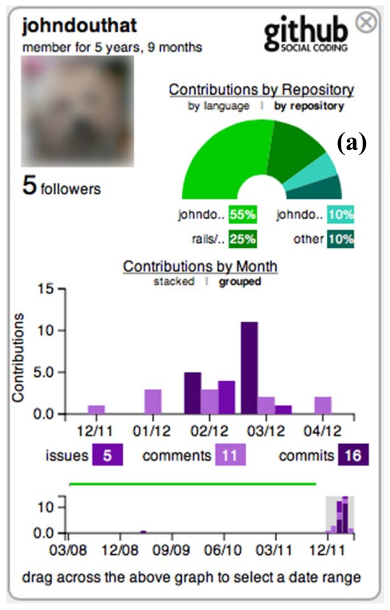
\includegraphics[width=4.5cm]{contributions.png}
  \caption{Visual Resume screenshot showing the skills and contributions of a developer}
  \label{fig:visualResume}
\end{figure*}

\rulemajor{Rule 5: Develop forms of legitimate peripheral participation}

Legitimate peripheral participation (LPP) provides newcomers with opportunities to ease into a project
and learn the norms of the community through low-risk tasks,
(i.e., tasks that will not interrupt the community's utility)~\cite{lave1991,wenger1999}.
In order to be successful LPP must give newcomers an opportunity to engage in ways that add value to the community.
However,
in communities such as GitHub,
core activities such as committing code and submitting pull requests can be socially daunting for newcomers~\cite{steinmacher2015}.
One form of encouraging LPP on this platform could be to encourage newcomers to add an issue to a repository when they notice a bug.
Another form of LPP would be to join the dialogue on a recently submitted pull request.
These provide newcomers interactive opportunities to learn the norms of the community. 

Building multiple ways of participating in a community demonstrates the variety of approaches newcomers can take to join the community.
This further demonstrates that there's not just one way to make technical contributions.
For example,
the main form of interaction in the community on Stack Overflow is to ask a question and posting an answer.
For some users,
engaging in that type of interaction can present barriers including an intimidating community size and fear of negative feedback~\cite{ford2016}.
Thus, it is important to provide additional forms of participation.
On Stack Overflow, this is demonstrated through the ability to edit questions and answer without the restriction of reputation points.
Developing a pathway to participation can decrease the presence of barriers.
In studying the evolution of how content is formed in these communities~\cite{baltes2018},
newcomers can better understand the norms of a community and the best way to contribute~\cite{ford2018}.

\rulemajor{Rule 6: Make knowledge findable.}

When starting to contribute to a project,
newcomers need to learn their way around it.
However,
newcomers to software projects are like explorers who must orient themselves within an unfamiliar landscape~\cite{dagenais2010}.
Thus,
it is important to make sure that all necessary information is accessible
(or at least searchable)
by newcomers during their first steps.

Information that is spread out usually makes newcomers feel lost and disoriented.
Given the different possibilities of places to maintain information
(e.g., wikis, files in the repository, shared documents, old tweets or Slack messages, and email archives),
it is important to keep information about a specific topic consolidated in a single place
so that newcomers do not need to navigate multiple data sources to find what they need.
The literature has shown that organizing the information make newcomers more confident and oriented~\cite{steinmacher2016}.
This organization is something important for technical and process documentation but also for communication channels.
Another suggestion is, therefore, to stick to a small number of communication channels
and to clearly define the goals for each of them.

At the same time,
outdated documentation may lead newcomers to a wrong understanding of the project,
which is also demotivating.
While it may be hard to keep documentation up-to-date,
community members should remove outdated information or, at least, clearly identify it as outdated.
Making newcomers aware of the absence or the status of a document can save their time and set their expectations.
By recognizing the obsolescence of the information,
communities may request help from the newcomers as a way to foster their contribution.

\rulemajor{Rule 7: Use opportunities for in-person interaction, but with caution.}

Open source software projects often rely heavily on remote workers communicating via text, audio, and video.
Research on face-to-face and audio/video-mediated communication is mixed
with regard to their comparative effectiveness~\cite{doherty1997,gallupe1990,nardi2002},
but demonstrates that each form has benefits and drawbacks.
In-person interaction is valuable for uninterrupted, synchronous dialog
and helps to establish mutual understanding in a streamlined way~\cite{omalley1996}.
Projects can therefore benefit from engaging newcomers in in-person interaction from time to time.

According to Huppenkothen and colleagues~\cite{huppenkothen2018},
newcomers may particularly benefit from hackweeks that,
``{\ldots}combine structured periods focused on pedagogy
(often with an emphasis on statistical and computational techniques)
and less structured periods devoted to hacks and creative projects,
with the goal of encouraging collaboration and learning among people at various stages of their career.''
Building newcomer-friendly events and activities into a hackweek
might serve as an effective approach for acclimating newcomers to the project and its community
as well as highlight the potential avenues for newcomer contributions.

However,
projects should exercise caution when asking newcomers to communicate in person.
First, potential contributors might shy away from the project if they are introverted,
suffer from social anxiety,
or have had bad experiences in the past in face-to-face settings.
Establishing and publicizing a Code of Conduct helps allay these concerns,
but some newcomers may still feel uncomfortable in group settings.
In this case,
not going to a meetup may leave them feeling less a part of the community.

Face-to-face communication also involves forms of information exchange
that are not easily captured and archived for all project members to see.
For example,
collocated project members might hash out ideas on whiteboards,
by scribbling notes,
or through informal chats.
Even when transcribing and/or taking photos of these is possible,
important contextual information may be lost~\cite{cherubini2007}.
Decisions and changes may seem to come out of nowhere when evaluated by a non-attendee,
so project leads should develop universally-accessible ways to communicate and explain the results of in-person activities.

\rulemajor{Rule 8: Provide an easy, complete, and up-to-date guide to contributing.}

For any form of organized activity,
it is likely more constructive and efficient to teach and reward desired behaviors than to change problematic behaviors down the line.
Project decision-makers can prompt desired practices in open source software development
by providing newcomers with ``how to contribute'' guidelines in easy-to-find, readily-available places.
Many projects follow GitHub's recommendation for placing such information in a CONTRIBUTING.md file~\cite{github-rec}.
Other projects,
such as the Apache Open Office Suite and rOpenSci,
provide text-based newcomer manuals and learning modules accessed through a web interface~\cite{apache-guidelines,ropensci-guidelines}.
Still, others take a more interactive approach,
such as the GNOME project's Newcomers Guide~\cite{gnome-newcomers},
which walks potential contributors through the contribution pipeline:
choosing a project,
acquiring and installing the necessary computing tools,
finding problems or choosing issues to work on,
submitting changes,
and following up on feedback.

``How to contribute'' guidelines,
no matter the form of presentation,
serve several additional purposes alongside describing expected contribution behaviors.
Contribution guidelines offer a centralized, well-organized description of resources
that a newcomer can consult while learning to navigate the project's technical and social environments~\cite{zanatta2017}.
Indeed, the social environment is a key constraint on newcomer behaviors~\cite{steinmacher2015};
explicitly-stated definitions of contribution expectations can ease newcomers' hesitancies
about whether or not their work is sufficient and suitable for the project.
Relatedly,
guidelines also acclimate newcomers to the norms of work and communication,
particularly when items such as necessary computing tools and codes of conduct are foregrounded.
In sum,
when combined with a welcoming, inclusive environment,
clear expectations about legitimate participation,
and shared software development goals,
contribution guidelines can help newcomers feel they are on equal footing with veteran project members.

Project decision-makers should keep in mind, however, 
that their perceptions of what constitutes clear, easy-to-find contribution guidelines
may not align with the perceptions of the newcomers themselves.
Continual reevaluation of the guidelines based on community member feedback is essential
to ensuring that contribution guidelines are achieving desired effects
and do not fall out of date (e.g., as technical and social elements of the community change).
In this sense,
contribution guidelines should be treated as living, evolving documents rather than immutable rules.

\rulemajor{Rule 9: make it easy for newcomers to start working.}

There is a lot to be gained from automating as much of your setup process you can
and thoroughly documenting whatever you can't. 
This critical special case of the previous rule is so important that it deserves to be a rule on its own.
The experience of getting set up to work on a project---the moment they go from ``I want to help''
to ``I'm able to help'' to ``I'm helping''---is often a contributor's first impressions of 
the experience of participating in that community.
This makes the developer setup process a critical moment in your relationship with every new contributor,
which in turn means that any complexity or confusion at this point is a significant barrier to participation.
In short, by treating the process of getting involved with the same care and attention you give
to the product itself, you're making it clear that you value those contributors' time and effort.

This work does not just benefit newcomers:
it also helps retention of existing intermittent contributors and the same work that makes your project more
accessible to new contributors today will do the same for future you.
Wheelchair ramps and the buttons that open heavy doors are not just used by those in wheelchairs:
they are just as helpful to people with strollers or one too many bags of groceries.
None of us are ever more than a sprained ankle away from desperately wanting that wheelchair ramp to be there.
In that same vein, a drive failure will someday force you to download a gigabyte of data
and reinstall some software, inevitably at the least convenient moment imaginable. 

\rulemajor{Rule 10: Follow up on success.}

Once a new contributor has been able to carry their first contribution over the line, 
you're likely to have a sense of their strengths and weaknesses.
This is then a good time to invite them to continue their involvement in your project.

The first and most important thing is to thank them for their contribution.
Gratitude and recognition are the most powerful tools available for community builders and maintainers. 
After that,
consider what you've learned of this contributor to help them find
the next issue they might want to work on.
If we have aspirations for our open source projects as a welcome and empowering community,
it is important that this be an invitation,
not a suggestion or demand. 

\bibliography{rules}

\end{document}
